\documentclass[a4paper,12pt,hidelinks]{report}

%%Pacchetti utili anche se non necessari

\usepackage{amsfonts}
\usepackage{amsmath}
\usepackage{latexsym}
\usepackage{tabularx}
\usepackage[italian]{babel}
\usepackage[bookmarks=true]{hyperref}
\usepackage{url}
% \usepackage{subfigure}
\usepackage{epstopdf}
\usepackage[utf8]{inputenc}
% \usepackage[utf8x]{inputenc}
\usepackage{listings}
\usepackage{graphicx}
%-------------------------------------------

% \title{Progettazione sito web\\ ''B\&B La Vecchia Posta''}
% \author{Daniele Di Pompeo \\mat. 226766}
% \annoaccademico{2013-2014}
\begin{document}
  \begin{titlepage}
    \begin{center}
    % Upper part of the page
      
\includegraphics[width=0.5\textwidth,keepaspectratio=true]{../img/logo}\\[1cm]    
      \textsc{\LARGE Covalide prototipo di navigazione}\\[0.6cm]
      \textsc{\LARGE  progetto del sito:\\[0.5cm] ``B\&B La Vecchia Posta''}\\ [2.0cm]

    % Author and supervisor
      \begin{minipage}{0.8\textwidth}
	\begin{flushleft} \large
	  \emph{Autore:} Daniele Di Pompeo \\[0.5cm]
	  \emph{Versione documento: 1.0}\\[0.5cm]
	  \emph{Data emissione del documento: \today}\\[0.5cm]
	\end{flushleft}
      \end{minipage}
    \end{center}
  \end{titlepage}

% \tableofcontents
 
\begin{abstract}
 In questo documento vengono elencate le peculiarità di navigazione del sito web in oggetto che sono state descritte nel documento dei requisiti in allegato
 alla documentazione rilasciata al committente.
 Il prototipo di navigazione è raggiungibile all'indirizzo \url{http://www.vecchiaposta.it/progettazione/index.html}.
 \par Il documento si riverisce al prototipo di navigazione, quindi si mostrano le considerazioni finali sui requisiti tecnici individuati nel relativo documento.
 Il tema presentato nel prototipo fornisce all'utente tutti gli strumenti per testarne l'usabilità, fornendo una reale e quasi totale navigazione del sito.
\end{abstract}

\section*{Layout generale}
Il protipo del layout utilizzato per la realizzazione del sito web è stato sottoposto al test di usabilità di vari tipi di utenti.
Ai vari utente sono state poste le seguenti domande:
\begin{itemize}
 \item Potresti raggiungere la sezione delle camere?
 \item Sei interessato alle attività proposte, sai raggiungere la sezione del sito?
 \item Riesci a scoprire gli eventi che ci sono nella zona?
 \item Cosa per te deve essere aggiunto o eliminato?
\end{itemize}
All'ultima domanda il test non è riuscito a fornire una risposta dettagliata essendo il prototipo presentato è completamente spoglio del comparto grafico.

\begin{itemize}
 \item \textbf{Utente esperto}: l'utente esperto ci ha fornito un feedback positivo sia per quanto riguarda lo stile del sito sia per la facile navigazione tra le sezione
 dello stesso. In particolare è riuscito subito a raggiungere la sezione desiderata ed ha apprezzato la struttura delle pagine.
 \item \textbf{Navigatore esperto}: facendo utilizzare il prototipo del sito web ad un navigatore esperto (utente che trascorre alcune ore giornaliere su internet), il sito 
 risulta essere abbastanza navigabile non potendo suggerire migliorie sul comparto grafico il test verrà riproposto a sviluppo ultimato.
 \item \textbf{Navigatore inesperto}: forse il test più importante per assicurare la buona riuscita della progettazione del sito. I risultati ottenuti si possono considerare 
 accetabili in relazione al nostro utente. 
 \par Il sito è risultato navigabile nella sua quasi totalità. L'utente non ha avuto grandi difficoltà nel effettuare le operazioni richieste.
\end{itemize}
Per completezza di informazioni si allega il video dell'utilizzo del prototipo da parte dell'utente medio, consultabile all'indirizzo \url{http://youtu.be/_KEx4eMBWiU}, che risulta raggiungere i prorpri obiettivi rapidamente senza 
problematiche.
\par Nelle successive fase di sviluppo si effettueranno test successivi mostrando all'utente il tema completo.

\section*{Struttura dei menu}
La struttura del menu risulta essere completamente visibile sia alla risoluzione scelta per la progettazione, sia ad una risoluzione più bassa.
Sono stati evitati scroll orizzontali nelle risoluzioni 1024px (\ref{fig:nav1024}) e 1200px (\ref{fig:nav1200}) (risoluzione di base) che coprono quasi la totalità 
delle configurazioni degli utenti che navigano su internet non attraverso dispositivi mobile.
\\Per quanto riguarda risoluzioni più basse e dispositivi mobile, si rimanda ad una versione successiva dello sviluppo.
\par La struttura del menu mantiene una proporzionalità accettabile con i contenuti informativi in entrambe le risoluzioni considerate. 
\\Si mostrano due screenshot alle due risoluzioni.
\begin{figure}[h!]%
    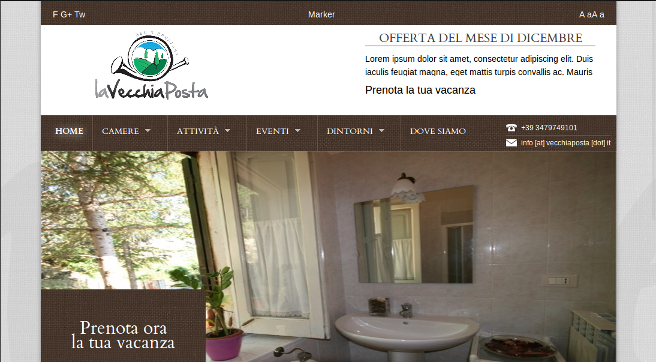
\includegraphics[width=0.9\textwidth,keepaspectratio=true]{../img/nav1024}
    \centering
    \caption{Prototipo: risoluzione 1024px}%
    \label{fig:nav1024}%
\end{figure}

\begin{figure}[h!]%
    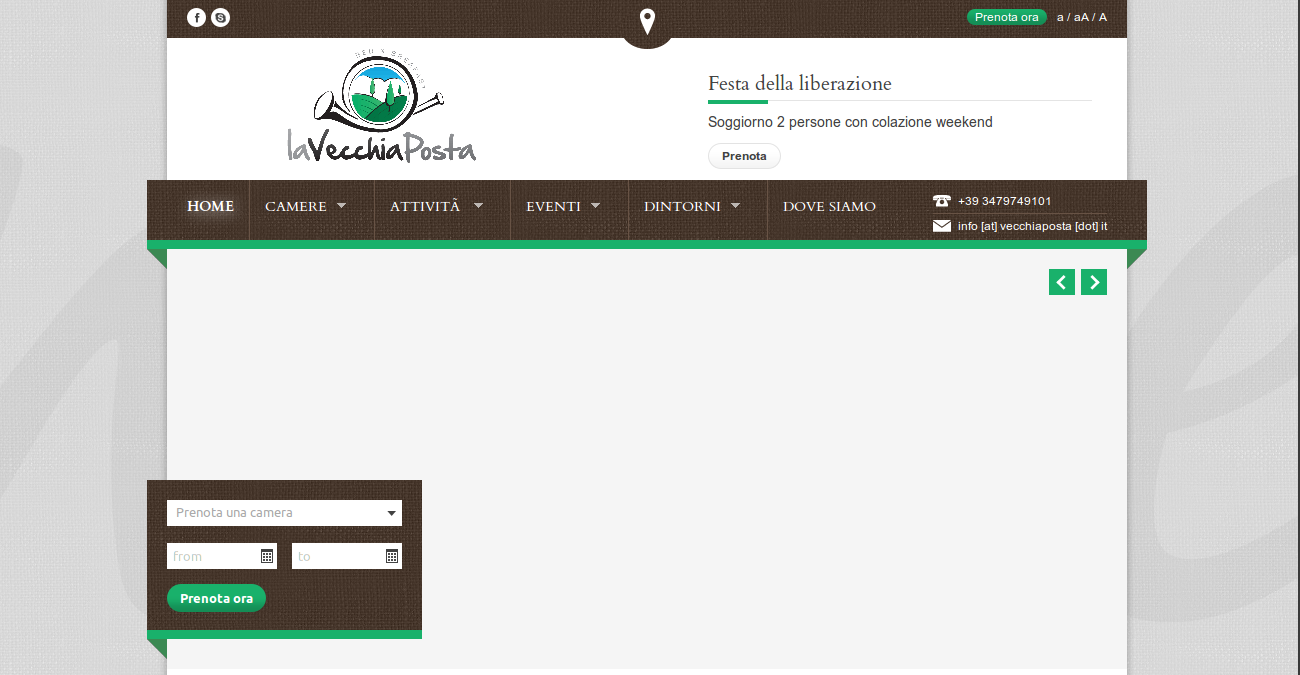
\includegraphics[width=0.9\textwidth,keepaspectratio=true]{../img/nav1200}
    \centering
    \caption{Prototipo: risoluzione 1200px}%
    \label{fig:nav1200}%
\end{figure}

\newpage
\section*{Navigazione}
Per la progettazione delle gabbie laogiche ci si è concentrati nello sviluppo di una struttura delle pagine che consenta di essere ripetibile nelle varie sezioni.
\par Le sotto sezioni sono state strutturate in modo tale da avere sopra la piega tutte le informazioni utili alla navigazione. In alto a sinistra si è inserito un'area 
destinata a contenere uno slider per le immagini relative alla pagina o a contenere la mappa stradale. Parallelamente il lato destro è stato utilizzato per 
fornire all'utente informazioni utili sottoforma di lista puntata e una scorciatoia alla prenotazione.
\\Sotto la piega si è riportata la descrizione dettagliata della sezione.
 \par In ogni modo la struttura del sito grazie alla ripetizione porta l'utente utilizzatore a non perdersi mantenendo alto lo stile dello stesso.

\section*{Etichette}
Nel documento dei requisiti, in allegato alla documentazione, alla sezione 2.1.1 \textit{Architettura informativa}, sono state individuate alcune aree semantiche 
che dovevano essere inserite nel sito. Si è scelto di mantenere la stessa struttura nelle etichette del menu perchè non si riscontrano problematiche di 
incoerenza e/o possibili incomprensioni. 
Dalle etichette del menu l'utente ha da subito una chiara visione di quale sia la sezione semantica su cui si sta dirigendo. 

\section*{Compatibilità browser}
Il sito web risulta essere compatibile con i principali browser sul mercato in particolare è stato testato su:
\begin{itemize}
 \item Chrome
 \item Firefox
 \item Opera
 \item Internet Explorer 10
\end{itemize}

\end{document}          